ในการพัฒนาโมเดลปัญญาประดิษฐ์สำหรับจำแนกการกระทำของมนุษย์นั้นมีพื้นฐานมาจากการจำแนกวัตถุ (object classification)
หมายถึงการใช้รูปภาพหนึ่งรูปในการประมวลผลและทำนายออกมาว่าภายในรูปนั้นมีบริบทการกระทำอย่างไร โดยไม่ได้คำนึงถึงข้อมูลเชิงต่อเนื่อง (spatio-temporal information)
จากบทความ "Quo Vadis, Action Recognition? A New Model and the Kinetics Dataset"\textsuperscript{\cite{I3D}} นั้นได้พัฒนาโครงสร้างของโมเดลปัญญาประดิษฐ์ (architecture) 
ที่มีประสิทธิภาพในการประมวลผลภาพเคลื่อนไหวได้ชื่อว่า I3D หรือ inflated 3D-convolution network
โดยโครงสร้างพื้นฐานของ I3D นั้นมาจาก Inception-v1\textsuperscript{\cite{Inception}} ที่ถูกพัฒนาโดย Goggle ซึ่งเป็นโครงสร้างที่มีประสิทธิภาพสูงในการจำแนกวัตถุในรูปภาพ
แล้ว I3D นั้นได้ทำการขยายมิติของโครงสร้างจาก 2 มิติ เป็น 3 มิติ เพื่อให้โมเดลปัญญาประดิษฐ์สามารถเรียนรู้ข้อมูลเชิงต่อเนื่องได้
\begin{figure}[!ht]
    \centering
    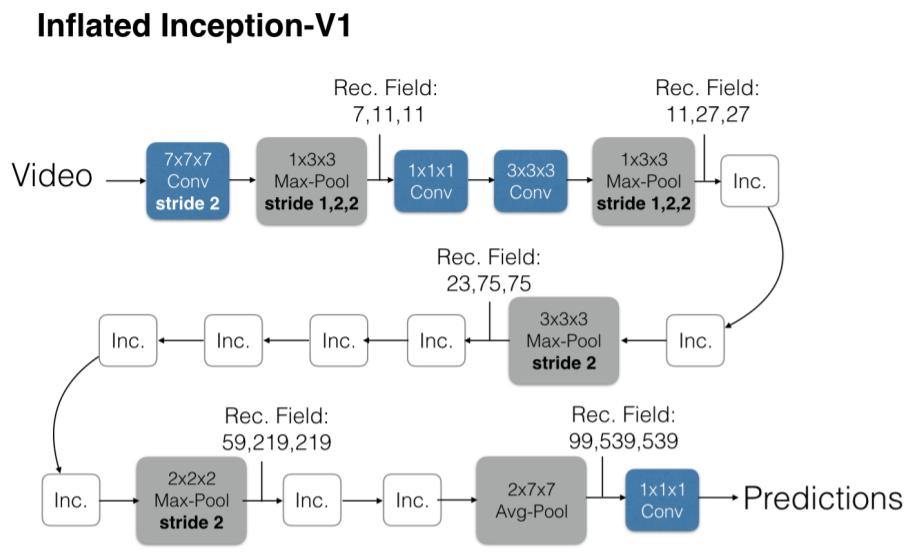
\includegraphics[width=1.0\textwidth]{chapter2/images/I3D.png}
    \caption{โครงสร้างของโมเดลปัญญาประดิษฐ์ I3D\textsuperscript{\cite{I3D}}}
    \label{fig:I3DArch}
\end{figure}
\clearpage
\begin{figure}[!ht]
    \centering
    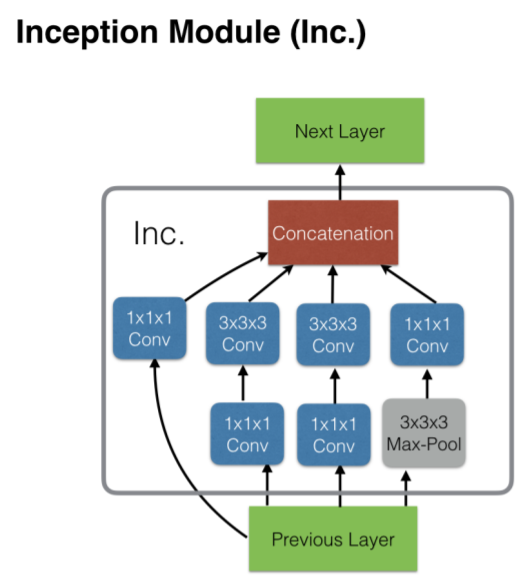
\includegraphics[width=0.5\textwidth]{chapter2/images/inceptionModule.png}
    \caption{โครงสร้างของโมเดลปัญญาประดิษฐ์ I3D\textsuperscript{\cite{I3D}}}
    \label{fig:InceptionModule}
\end{figure}

ประสิทธิภาพของโมเดล I3D แบบ two-stream เมื่อเทียบกับ long-short term memory (LSTM),
3D-convolution network, two-stream และ 3D-fused โดยใช้เครื่องมือในการวัดผลคือ Top@1 accuracy ตามตารางที่ \ref{tab:I3DPerformance}
\begin{table}[!ht]
    \begin{tabular}{|*{10}{c|}}
        \hline
        \multirow{2}{*}{Architecture} & \multicolumn{3}{c|}{UCF-101} & \multicolumn{3}{c|}{HMDB-51} & \multicolumn{3}{c|}{Kinetics}\\
        \cline{2-10}
            & RGB & Flow & RGB + Flow & RGB & Flow & RGB + Flow & RGB & Flow & RGB + Flow\\
        \hline\hline
        LSTM            & 81.0 & – & – & 36.0 & – & – & 63.3 & – & –\\
        3D-ConvNet      & 51.6 & – & – & 24.3 & – & – & 56.1 & – & –\\
        Two-Stream      & 83.6 & 85.6 & 91.2 & 43.2 & 56.3 & 58.3 & 62.2 & 52.4 & 65.6\\
        3D-Fused        & 83.2 & 85.8 & 89.3 & 49.2 & 55.5 & 56.8 & – & – & 67.2\\
        Two-Stream I3D  & 84.5 & 90.6 & 93.4 & 49.8 & 61.9 & 66.4 & 71.1 & 63.4 & 74.2\\
        \hline
    \end{tabular}
    \caption{ประสิทธิภาพของโมเดล I3D แบบ two-stream เมื่อใช้ข้อมูลจาก UCF-101, HMDB-51 และ Kinetics ในการสร้างและทดสอบด้วยเครื่องมือวัดผลแบบความแม่นยำจากการทำนายอันดับแรกสุด}
    \label{tab:I3DPerformance}
\end{table}